% **************************************************
% Document Class Definition
% **************************************************
\documentclass[%
	paper=A4,					% paper size --> A4 is default in Germany
	%	twoside=true,
	twoside=false,				% onesite or twoside printing
	openright,					% doublepage cleaning ends up right side
	parskip=full,				% spacing value / method for paragraphs
	chapterprefix=true,			% prefix for chapter marks
	11pt,						% font size
	headings=normal,			% size of headings
	bibliography=totoc,			% include bib in toc
	listof=totoc,				% include listof entries in toc
	titlepage=on,				% own page for each title page
	captions=tableabove,		% display table captions above the float env
	draft=false,				% value for draft version
]{scrreprt}%

% **************************************************
% Debug LaTeX Information
% **************************************************
%\listfiles

% **************************************************
% Information and Commands for Reuse
% **************************************************
\newcommand{\thesisTitle}{Designing and implementing a system for passive user feedback}
\newcommand{\thesisName}{Janis Krasemann}
\newcommand{\thesisSubject}{Proposal}
\newcommand{\thesisDate}{November 29, 2017}
\newcommand{\thesisVersion}{0.3}

\newcommand{\thesisFirstReviewer}{Dr. Simon Oberth\"ur}
\newcommand{\thesisFirstReviewerUniversity}{\protect{Paderborn University}}
\newcommand{\thesisFirstReviewerDepartment}{Software Innovation Campus Paderborn}

\newcommand{\thesisSecondReviewer}{John Doe}
\newcommand{\thesisSecondReviewerUniversity}{\protect{Paderborn University}}
\newcommand{\thesisSecondReviewerDepartment}{Software Innovation Campus Paderborn}

\newcommand{\thesisFirstSupervisor}{Bj\"orn Senft}
\newcommand{\thesisSecondSupervisor}{Dr. Simon Oberth\"ur}

\newcommand{\thesisUniversity}{\protect{Paderborn University}}
\newcommand{\thesisUniversityDepartment}{Faculty for Computer Science, Electrical Engineering and Mathematics}
\newcommand{\thesisUniversityInstitute}{Computer Science}
\newcommand{\thesisUniversityGroup}{Database and Information Systems}
\newcommand{\thesisUniversityCity}{Paderborn}
\newcommand{\thesisUniversityStreetAddress}{Warburger Stra{\ss}e 100}
\newcommand{\thesisUniversityPostalCode}{33098}

% **************************************************
% Load and Configure Packages
% **************************************************
\usepackage[utf8]{inputenc}		% defines file's character encoding
\usepackage[english]{babel} % babel system, adjust the language of the content
\usepackage[					% clean thesis style
	figuresep=colon,%
	sansserif=false,%
	hangfigurecaption=false,%
	hangsection=true,%
	hangsubsection=true,%
	colorize=full,%
	colortheme=bluemagenta,%
	bibsys=bibtex,%
	bibfile=bib-refs,%
	bibstyle=alphabetic,%
]{cleanthesis}
% JK Custom setup
\usepackage{todonotes}
\usepackage[printonlyused]{acronym}
% !TEX root = ./thesis.tex
%
\acrodef{CQRS}{Command Query Responsibility Segregation}
\acrodef{EDSD}{experiment-driven software development}
\acrodef{CSE}{Continuous Software Engineering}
\acrodef{REST}{Representational State Transfer}
\acrodef{SQL}{Structured Query Language}
\acrodef{CQL}{Cassandra Query Language}
\acrodef{DSL}{Domain Specific Language}
\acrodef{YAML}{YAML Ain't Markup Language}
\acrodef{VM}{Virtual Machine}
\acrodef{CLI}{Command Line Interface}
\acrodef{RSS}{Rich Site Summary}
\acrodef{API}{Application Programming Interface}
\acrodef{TCP}{Transmission Control Protocol}
\acrodef{UDP}{User Datagram Protocol}
\acrodef{HTTP}{Hypertext Transfer Protocol}
\acrodef{XHR}{XMLHttpRequest}
\acrodef{SPA}{Single-Page Application}
\acrodef{UX}{User Experience}
\acrodef{IFAS}{Implicit Feedback Analysis System}
\acrodef{HTML}{Hypertext Markup Language}
\acrodef{OSI}{Open Systems Interconnect}
\acrodef{JSON}{JavaScript Object Notation}

\usepackage[noabbrev]{cleveref}

\hypersetup{					% setup the hyperref-package options
	pdftitle={\thesisTitle},	% 	- title (PDF meta)
	pdfsubject={\thesisSubject},% 	- subject (PDF meta)
	pdfauthor={\thesisName},	% 	- author (PDF meta)
	plainpages=false,			% 	-
	colorlinks=false,			% 	- colorize links?
	pdfborder={0 0 0},			% 	-
	breaklinks=true,			% 	- allow line break inside links
	bookmarksnumbered=true,		%
	bookmarksopen=true			%
}

% **************************************************
% Document CONTENT
% **************************************************
\begin{document}

% --------------------------
% rename document parts
% --------------------------
%\renewcaptionname{ngerman}{\figurename}{Abb.}
%\renewcaptionname{ngerman}{\tablename}{Tab.}
\renewcaptionname{english}{\figurename}{Fig.}
\renewcaptionname{english}{\tablename}{Tab.}

% --------------------------
% Front matter
% --------------------------
\pagenumbering{roman}			% roman page numbing (invisible for empty page style)
\pagestyle{empty}				% no header or footers
% !TEX root = ../thesis.tex
%
% ------------------------------------  --> cover title page
\begin{titlepage}
	\pdfbookmark[0]{Cover}{Cover}
	\flushright
	\hfill
	\vfill
	{\LARGE\thesisTitle \par}
	\rule[5pt]{\textwidth}{.4pt} \par
	{\Large\thesisName}
	\vfill
	\textit{\large\thesisDate}	
\end{titlepage}


% ------------------------------------  --> main title page
\begin{titlepage}
	\pdfbookmark[0]{Titlepage}{Titlepage}
	\tgherosfont
	\centering

	{\Large \thesisUniversity} \\[4mm]
	
\includegraphics[width=12cm]{gfx/UPB-Logo.png} \\[2mm]
	\textsf{\thesisUniversityDepartment} \\
	\textsf{\thesisUniversityInstitute} \\
	\textsf{\thesisUniversityGroup} \\

	\vfill
	{\large \thesisSubject} \\[5mm]
	{\LARGE \color{ctcolortitle}\textbf{\thesisTitle} \\[10mm]}
	{\Large \thesisName} \\

	\vfill
	\begin{minipage}[t]{.27\textwidth}
		\raggedleft
		\textit{1. Reviewer}
	\end{minipage}
	\hspace*{15pt}
	\begin{minipage}[t]{.65\textwidth}
		{\Large \thesisFirstReviewer} \\
	  	{\small \thesisFirstReviewerDepartment} \\[-1mm]
		{\small \thesisFirstReviewerUniversity}
	\end{minipage} \\[5mm]
	\begin{minipage}[t]{.27\textwidth}
		\raggedleft
		\textit{2. Reviewer}
	\end{minipage}
	\hspace*{15pt}
	\begin{minipage}[t]{.65\textwidth}
		{\Large \thesisSecondReviewer} \\
	  	{\small \thesisSecondReviewerDepartment} \\[-1mm]
		{\small \thesisSecondReviewerUniversity}
	\end{minipage} \\[10mm]
	\begin{minipage}[t]{.27\textwidth}
		\raggedleft
		\textit{Supervisors}
	\end{minipage}
	\hspace*{15pt}
	\begin{minipage}[t]{.65\textwidth}
		\thesisFirstSupervisor\ and \thesisSecondSupervisor
	\end{minipage} \\[10mm]

	\thesisDate \\

\end{titlepage}


% ------------------------------------  --> lower title back for single page layout
\hfill
\vfill
{
	\small
	\textbf{\thesisName} \\
	\textit{Designing and Implementing a System for Passive User Feedback} \\
	\thesisSubject, \thesisDate \\
	Reviewers: \thesisFirstReviewer\ and \thesisSecondReviewer \\
	Supervisors: \thesisFirstSupervisor\ \\[1.5em]
	\textbf{\thesisUniversity} \\
	\textit{\thesisUniversityGroup} \\
	\thesisUniversityInstitute \\
	\thesisUniversityDepartment \\
	\thesisUniversityStreetAddress \\
	\thesisUniversityPostalCode\ and \thesisUniversityCity
}
		% INCLUDE: all titlepages
\clearpage

\pagestyle{plain}				% display just page numbers
% !TEX root = ../proposal.tex
%
\pdfbookmark[0]{Abstract}{Abstract}
\chapter*{Abstract}
\label{sec:abstract}
\vspace*{-10mm}

Because an increasing amount of computer engineers have been frustrated with failing software products due to the slow and inflexible phases of classical software engineering, alternative practices such as \emph{Continuous Software Engineering} have emerged and gained a lot of traction during the past decade.
In order to continuously improve a software system, reliable usage data from the user is needed.
%These experiments help the creators of a piece of software to test and validate their assumptions about a product and its features early in the development process.
%User feedback is the data upon which these experiments rely.
% What is the problem?
%The area of innovation via experimentation in the software industry is already well researched, but lacks a more holistic view on collecting, aggregating and analysing the passive user feedback needed for evaluating an experiment.
The area of Continuous Software Engineering is already well researched but lacks a more holistic view on collecting, aggregating and analyzing the user feedback needed for effectively improving the system.
%Why is this a problem?
%This is problematic because, although many companies realise the need for experimentation in their development process, they struggle with the systematic adoption of these practices.
This is problematic because, although many companies realize the need for continuity in their development process, they struggle with the systematic adoption of these practices.
%What is the / a solution?
By researching how to design and implement a system for establishing passive user feedback with considerably low effort, this thesis aims to fill this gap.
It is expected that event sourcing is a good fit for realizing such a system, which will be further investigated in the thesis.
%Event sourcing is a storage solution in which data is stored in the form of immutable event objects representing actions on business objects; in combination, all these events represent the application state.
Designing and implementing said system includes researching solutions for storing, aggregating and analyzing user feedback data.
A prototype using the chosen technologies is then implemented, which involves setting up and configuring various services as well as writing software that connects them.
The system is evaluated via a controlled experiment in order to validate the assumptions in this thesis.
%This will presumably involve either a user test for gathering passive user feedback, or analysing the user actions in an existing data set.
%The gathered data is then aggregated and analysed using the implemented system, and then compared with the results of a questionnaire with usability experts.
%Why is this a solution / what is ?
Practitioners in the software industry could use the system presented in the thesis as a reference for introducing collection and analysis of passive user feedback into their software, which facilitates the adoption of Continuous Software Engineering.
		% INCLUDE: the abstracts (english and german)
\clearpage
%
%% !TEX root = ../thesis-example.tex
%
\pdfbookmark[0]{Acknowledgement}{Acknowledgement}
\chapter*{Acknowledgement}
\label{sec:acknowledgement}
\vspace*{-10mm}

\Blindtext[2][2]
 % INCLUDE: acknowledgement
%\clearpage
%
\setcounter{tocdepth}{2}		% define depth of toc
\tableofcontents				% display table of contents
\clearpage

% --------------------------
% Body matter
% --------------------------
\pagenumbering{arabic}			% arabic page numbering
\setcounter{page}{1}			% set page counter
\pagestyle{maincontentstyle} 	% fancy header and footer

% !TEX root = ../thesis.tex
%
\chapter{Introduction}
\label{ch:intro}

% CONTEXT

% GAP

% INNOVATION

% copy from proposal:

Best practices in software development changed dramatically since its origins in the 1950's~\cite{boehm2006view}.
Software engineering in most of the 20th century was largely based on careful planning and specification and therefore rather slow-paced and inflexible.
Since twenty years, however, these plan-driven development methods have been frustrating many people because the influencing circumstances change more and more rapidly, not least due to the growing importance of the internet~\cite{Williams2003}.
A result of this rapid change of the environment is that product features, which were perfectly valid at the time of their envisioning, became outdated, irrelevant or otherwise undesirable while the feature was still being planned or implemented -- not to mention features that are in fact not desired by the customers in the first place.
This insight is often not gained until the feature is shipped to the customer.
As a consequence, short release cycles and fast customer feedback have steadily been growing in importance.
These values are emphasized in \acf{CSE}~\cite{Bosch2014}, which adopts and extends the principles from \emph{DevOps} and agile software development~\cite{Fitzgerald2017,fowler2001agile}.

Adopting the core premises of \ac{CSE} is considered to be a gradual process, which is represented by the \emph{Stairway to Heaven}~\cite{Olsson2012} (see~\cref{fig:stairway}).
Starting from classical software development, the next step is agile software development.
This step is followed by continuous integration and deployment, respectively. 
The last step in the Stairway to Heaven is "Research \& Development as an Innovation System".
This means that the continuity gained in the previous steps is used for frequently deploying changes to the customers.
These changes are then assessed by analyzing user feedback data which was previously gathered using active or passive methods.
While active user feedback, e.g. in form of surveys, can yield useful qualitative observations about the product, the fact that the user has to actively take time for giving their feedback is often problematic.
Passive user feedback avoids this problem by automatically collecting feedback while the user works with the system; an example for this is measuring the time a user needs to perform certain actions in the software.
An \emph{evolutionary system} as described here allows for quicker responses to market changes and more accurate estimation of customer needs.

\begin{figure}[htb]
        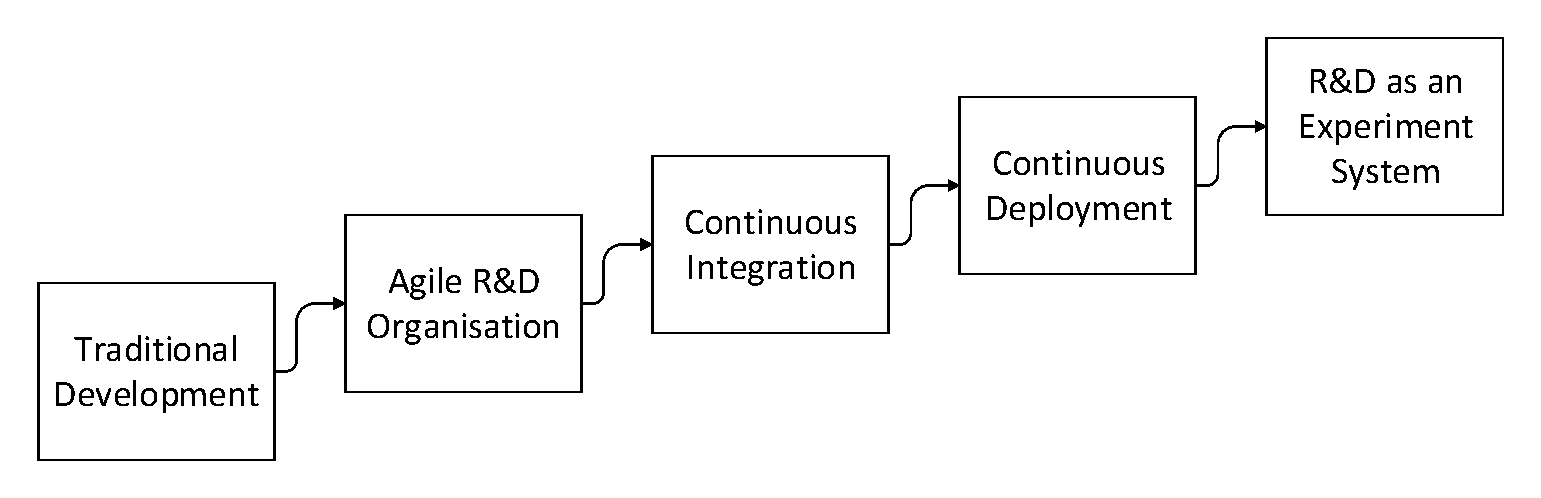
\includegraphics[width=\textwidth]{gfx/stairway.pdf}
        \caption{The "stairway to heaven" evolutionary model; adapted from~\cite{Olsson2012}.}
        \label{fig:stairway}
\end{figure}

%\cite{Bosch2014}

%The results of such an experiment are then used for deciding wether the feature should become a part of the final product.
%Thus, the goal in this case is to increase the effectiveness of developing a software product by implementing the \emph{right} features.
%Experiments are also used in order to compare different implementations of the same feature, thus improving the quality of an existing feature.
%This approach is contrary to the more classical software development methods, in which the stakeholders make certain assumptions which result in the envisioning of a feature, with feedback by a customer or stakeholder being given only much later in the development process~\cite{Bosch2012}.

%The core premise in innovation experiment systems is the continuous implementation and validation of assumptions about envisioned features via experiments in short sprints~\cite{Bosch2014}.
%The results of such an experiment are then used for deciding wether the feature should become a part of the final product.
%Thus, the goal in this case is to increase the effectiveness of developing a software product by implementing the \emph{right} features.
%Experiments are also used in order to compare different implementations of the same feature, thus improving the quality of an existing feature.
%This approach is contrary to the more classical software development methods, in which the stakeholders make certain assumptions which result in the envisioning of a feature, with feedback by a customer or stakeholder being given only much later in the development process~\cite{Bosch2012}.

The agile and continuous work methods in \ac{CSE} come with several implications for the system architecture and the company culture~\cite{Lindgren2015,Olsson2012}.
In particular, monolithic software systems are considered too cumbersome and slow to change; instead, small services that communicate with each other through a well defined but lightweight API are recommended.
\citet{ford2017building} argue that such distributed systems work well with the \emph{Parallel Model} concept introduced by \citet{WEB:Fowler:2005-2}.
The rationale is that using Parallel Model, services can work with their own specialized read model without interfering with or complicating the overall application state.
In order to make use of Parallel Model, it is recommended that the system also uses \emph{Event Sourcing}~\cite{WEB:Fowler:2005,WEB:Fowler:2005-2}.
Event sourcing is a storage solution in which data is stored in the form of immutable event objects representing actions on business objects; in combination, all these events represent the application state.
The most obvious advantage of this approach is that the event log represents a complete log of all transactions.
More importantly, however, this also allows for the execution of temporal queries which compute the application state at any given point in time, and the ability to replay events, possibly after modifying the application state at a certain point in time.
A consequence of event replayability is that events can be received in any given sequence, which otherwise is a common problem in asynchronous systems.

This thesis aims at taking a more holistic approach to the innovation system concept from \ac{CSE} by designing and implementing a system that allows for easy collection of passive user feedback (\cref{sec:intro:goals} describes the objectives in more detail).
The result will be a set of interacting services which provide the ability to collect, aggregate and analyze passive user feedback in order to facilitate innovation in the research and development process.
It is anticipated that this system will profit from the usage of even sourcing, but this has to be further investigated in the thesis.
The resulting system shall be called \ac{IFAS}.
It can be adopted by individuals and companies in the software industry who want to fully embrace \ac{CSE} and thus take the last step in the Stairway to Heaven.

% \cite{Bosch2012}: First, it is focused on continuously evolving the software by frequently deploying new versions. Second, customers and customer usage data play a central role throughout the development process. Third, development is focused on innovation and testing as many ideas as possible with customers to drive customer satisfaction and, consequently, revenue growth.

\section{Motivation}
\label{sec:intro:motivation}

TODO: explain that the developed system enables / improves: (cf. \cite{Bosch2012} figure 2) 

- AB testing, collecting metrics \& performance metrics (due to the functionality)

- can also be used in non-commercial deployment because of its flexibility and because its free!

- classify how the pre-dev, non-commercial and commercial deployment phases and the scopes (optimization, new features, new products) fit here

\begin{table}
\centering
\begin{tabular}{p{2.5cm}|p{3.2cm}p{3.2cm}p{3.2cm}}
 & \textbf{Pre-development} & \textbf{Non-commercial deployment} & \textbf{Commercial \newline deployment}  \\ \hline
Optimization & Ethnographic studies & Independently deployed extensions &\textit{ A/B testing}  \\
New features & Solution jams & Feature alpha & Instrumentation / \textit{collecting metrics}  \\
New products & Advertising\newline Mockups\newline BASES testing & Product alpha\newline Labs website & Surveys\newline Performance metrics 
\end{tabular}
\caption[The scope of innovation experiments by \citet{Bosch2012}.]{
The scope of innovation experiments by \citet{Bosch2012}.
\ac{IFAS}' functionality enables A/B testing and collecting metrics (\textit{italic}).
Because the system is free and due to its flexibility, it also potentially enables these for non-commercial deployments.
}
\end{table}

% Most techniques were based on eliciting direct customer feedback through familiar means such as stakeholder interviews and surveys, prototypes, usability and user experience testing, and other forms of user testing. Bug reports and feature voting were also used as a way to guide development. \cite{lindgren2015software}

% Focusing on products and features that create the most customer value was seen as a way to speed up development: ?I don?t think you can accelerate anything. What you can do is do less.? \cite{lindgren2015software}

%copy from proposal

The last step in the Stairway to Heaven of \acf{CSE} is introducing an innovation system, also referred to as an \emph{experiment system}~\cite{Olsson2012}.
Several companies have published their findings about experimentation in the software development process, in the form of scientific papers or blog posts.
Amongst others, Microsoft~\cite{Kohavi2013}, LinkedIn~\cite{Xu2015}, Google~\cite{Tang2010}, Facebook~\cite{Bakshy2014}, and Netflix~\cite{WEB:Netflix:2016} issued reports about best practices and pitfalls that they experienced, all concluding that introducing experimentation into the software development process benefits both the choice about which features to implement as well as their quality.
In addition, several authors have published scientific papers in which they propose models and architectures for experimental software development~\cite{Fagerholm2014,Fagerholm2017,Johanssen2017,Lindgren2015}.
Although practitioners in the software industry often claim that they embrace experimentation and innovation in their research and development process, these practices are still not fully adopted according to a study by \citet{lindgren2015software}.
Especially the systematic and continuous aspects of experimentation lack adoption.

% Problem f�r Motivation ist hier: Wenn ich nicht direkt auf Event Sourcing Bezug nehme (d.h. es offen lasse ob Event Sourcing verwendet wird oder nicht) wird der Scope zu gro�: "Wie kann an eine Experimentier-Plattform implementieren" haben andere Leute schon beantwortet.
While the overall area of experimentation in software development is thus well researched, most papers are either more of a report about specific best practices or a rather abstract description of an architecture.
The same applies to the paper that initially proposed the Stairway to Heaven concept~\cite{Olsson2012}.
This is problematic for potential applicants of \ac{CSE}, because while these reports are very practice-oriented, they lack a more general view on the problem at hand, and the other way around for the architecture-focused papers.
Therefore, the aim of this thesis is to bridge this gap and provide a more holistic view on collecting, aggregating and analyzing passive user feedback.
This will enable applicants to implement their own innovation / experiment systems as described in \ac{CSE}, based on a scientifically tested architecture.


\section{Objectives}
\label{sec:intro:objectives}

% copy from proposal

The goal of the thesis is to design, implement and validate a system for passive user feedback with a more holistic view of the problem than in existing publications.
Using this system, it shall be possible to visualize and analyze passive user feedback that was previously supplied to its storage layer.
In order to accomplish this task, a system with functionalities as pictured in \cref{fig:system:vision} has to be implemented.
The concrete objectives are as follows:

\begin{enumerate}
\item Classify existing solutions and approaches for establishing passive user feedback.
\item Design and implement a system that allows the collection of passive user feedback with considerably low effort.
This part of the system is comprised of the storage layer, an aggregation service and a hypothetical client application which logs events to storage whenever the user performs certain actions (cf. 4.).
%It also features two users: The end user of the client application, and the analyst who wants to evaluate the user feedback.
These events can be purely UI related, such as click or hover events, but can also be related to the business logic, like executing transactions or creating content.
In order to forward the user feedback data to the analysis application (cf. 3.), the aggregation service has to fetch the appropriate data from the store.
While making use of a caching mechanism during this step would certainly make sense, such a feature will presumably not be part of the final solution due to the additional complexity; if this is the case, the system shall be easily extensible for introducing such a feature.
This objective involves researching and assessing fitting infrastructure and tooling solutions.
\item Design and implement this system such that it also allows analysis of collected user feedback.
Feedback should be ready for analysis within at most a minute.
When someone wants to evaluate the collected user feedback via the analysis application, the application shall display the corresponding data in an appropriate format, which it fetches from the aggregation service.
The best approach for displaying the data has yet to be evaluated but will involve some graphical representation in form of charts and/or graphs.
This objective also implicates research and choosing of appropriate solutions that shall be used for this part of the system.
\item Evaluate how this system performs, which involves collecting user feedback and analyzing it.
Implementation of the client application itself will not be done for the purpose of this thesis.
Instead, some existing application shall be extended in order to log the appropriate events or an existing data set such as the one presented by \citet{Deka:2017:Rico} shall be used.
In the latter case, some application or script has to be written which imports the needed UI interaction data to the database.
\item As an additional requirement, the developed system shall be platform independent, i.e. run on the most widely used operating systems Linux, MacOS, and Windows.
\end{enumerate}

\begin{figure}[htb]
        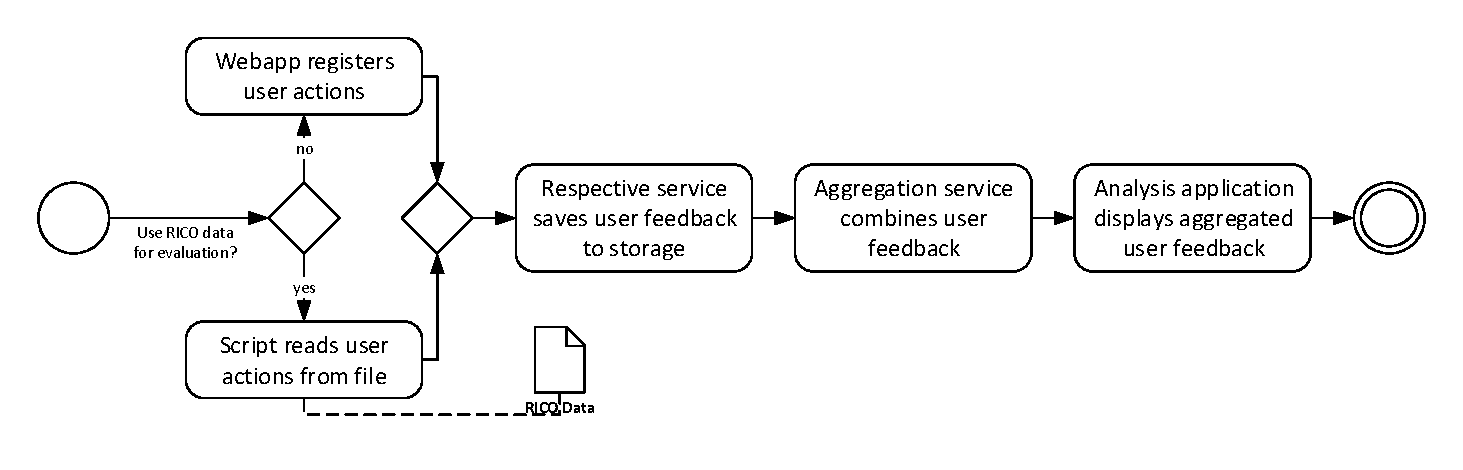
\includegraphics[width=1.1\textwidth]{gfx/architecture-3.pdf}
        \caption{The activities that the envisioned system is able to perform.}
        \label{fig:system:vision}
\end{figure}

%\section{Motivation and Problem Statement}
%\label{sec:intro:motivation}

\section{Approach}
\label{sec:intro:approach}

% copy from proposal

In order to achieve the objectives described in \cref{sec:intro:goals}, the working time of the thesis will roughly be divided into three segments: Research, implementation, and evaluation.
Putting the gained findings into writing is part of each of these segments.

Part of the research phase will be dedicated to reading up on the central topics for this thesis, namely but not exclusively \acf{CSE}, event sourcing, \acf{CQRS} and passive user feedback as well as methods for collecting it.
Aside from that, some decisions regarding the architecture and technology require additional research.
This involves researching, comparing and finally choosing an appropriate storage solution.
Current findings suggest that an event store, and in particular the Event Store reference implementation\footnote{\url{https://eventstore.org/}}, is a good fit for this.
The advantages of using event sourcing in this context are as follows:

\begin{enumerate}
\item Event replayability could be used to further mitigate the risk of creating experimental features: If a change in the software causes some faulty event to be created, it can later be modified or deleted.
Incorrect changes that are based on this faulty event can automatically be corrected using the Retroactive Event technique~\cite{WEB:Fowler:2005-3}.
Contrary to classical relational databases, the overall application state in an event store would not be corrupted by this.
It would also be possible to create separate event stores just for specific features, which could later be applied to the main event store by replaying the events from the experimental store.
\item When a feature has to be analyzed, temporal queries could be used for retrieving all events in a specific time frame.
\item Event sourcing and \ac{CQRS} advocate a distributed system architecture -- which is also true for the evolutionary systems present in \ac{CSE}~\cite{ford2017building}.
\end{enumerate}

In particular, the temporal query feature could render additional aggregation services obsolete.
Additional backup systems that roll back changes issued by potential experiments could also possibly be removed because of an event stores inherent ability to roll back and redo changes.
These assumptions would have to be validated over the course of the actual thesis.

A solution for aggregating the data has to be researched; the aforementioned temporal query feature is one candidate for this, another is Elasticsearch\footnote{\url{https://www.elastic.co/}}.
This aggregation service has to be paired with some service or application that analyses the generated data; Kibana\footnote{\url{https://www.elastic.co/products/kibana/}} seems to be a promising solution.
In order to achieve high platform independence and flexibility, a container platform such as Docker\footnote{\url{https://www.docker.com/}} will be used which also requires some research.
In order to be able to decide whether to use the RICO dataset~\cite{Deka:2017:Rico} instead of a custom client application for the evaluation part, this dataset will have to be assessed further.

The first task in the implementation phase will be to finalize the system architecture.
While the architecture is not expected to be overly complex and the first draft of its capabilities already exists at the time of writing (cf. \cref{fig:system:vision}), some alterations are possible and expected.
This task also involves deciding which data to save to the storage layer and which logical structure this data has to have.
When the system architecture design is finalized, the actual implementation can begin, which first of all involves setting up and configuring the storage solution.
If user feedback data is to be generated from a client application and not using the RICO dataset, the actual feedback logging has to be implemented as well.
Depending on the choice of aggregation service, if any, this service also has to be set up and/or implemented; the same holds for the analysis solution.

Finally, the implemented solution will be evaluated by executing up to two experiments.
The first experiment for the evaluation will be a questionnaire in which usability experts answer questions about a given application.
The results of the questionnaire will be compared to the passive user feedback data of the given application.
Depending on the means of collecting this user data, an experiment for collecting this data has to be designed and executed with some test subjects; this is not necessary if the RICO dataset is chosen as the source of user data.
The experiments have to be planned and executed carefully in order to have high internal and external validity~\cite{Huitt2010}.
Existing studies about best practices and pitfalls of running controlled experiments can be useful here~\cite{Kohavi2009}.


\section{Thesis Structure}
\label{sec:intro:structure}

\todo{Paragraphen zusammenziehen oder mehr schreiben}

In the fundamentals (\ref{ch:fundamentals}), the topics that are required to understand the contents of this thesis are explained.

The related work chapter (\ref{ch:related-work}) deals with scientific papers which have already explored the topics of passive user feedback and \ac{CSE} to some degree.

The first step to doing the design and implementation of the passive feedback system was to explore, evaluate and classify existing solutions for data storage, aggregation and analysis.
This is described in the Classifications chapter (\ref{ch:classifications}).

After choosing the technology for the implementation, various design decisions had to be made, which are explained in the System Design chapter (\ref{ch:design}).

The actual implementation details are then described in the subsequent chapter (\ref{ch:implementation}).

Upon finishing the implementation, the system was evaluated by a user and an expert survey, the methods and results of which are explained in the evaluation chapter (\ref{ch:evaluation}).

Possibilities for future work are given in its own chapter (\ref{ch:future-work}), followed by the conclusion (\ref{ch:conclusion}).

The appendix contains source code and configuration files of the various applications and services that were implemented and used.

% !TEX root = ../thesis-example.tex
%
\chapter{Concepts: This text is here to test a very long title, to simulate the line break behavior, to show that an extremely long tilte also works}
\label{sec:concepts}

\cleanchapterquote{Users do not care about what is inside the box, as long as the box does what they need done.}{Jef Raskin}{about Human Computer Interfaces}

\Blindtext[2][1]

\section{Concepts Section 1}
\label{sec:concepts:sec1}

\Blindtext[2][2]

\section{Concepts Section 2}
\label{sec:concepts:sec2}

\Blindtext[3][2]

\section{Concepts Section 3}
\label{sec:concepts:sec3}

\Blindtext[4][2]

\section{Conclusion}
\label{sec:concepts:conclusion}

\Blindtext[2][1]

% !TEX root = ../thesis-example.tex
%
\chapter{System}
\label{sec:system}

\cleanchapterquote{Innovation distinguishes between a leader and a follower.}{Steve Jobs}{(CEO Apple Inc.)}

\Blindtext[2][1]

\section{System Section 1}
\label{sec:system:sec1}

\Blindtext[1][2]

\begin{figure}[htb]
	\includegraphics[width=\textwidth]{gfx/Clean-Thesis-Figure}
	\caption{Figure example: \textit{(a)} example part one, \textit{(c)} example part two; \textit{(c)} example part three}
	\label{fig:system:example1}
\end{figure}

\Blindtext[1][2]

\section{System Section 2}
\label{sec:system:sec2}

\Blindtext[1][2]

\begin{figure}[htb]
	\includegraphics[width=\textwidth]{gfx/Clean-Thesis-Figure}
	\caption{Another Figure example: \textit{(a)} example part one, \textit{(c)} example part two; \textit{(c)} example part three}
	\label{fig:system:example2}
\end{figure}

\Blindtext[2][2]

\section{System Section 3}
\label{sec:system:sec3}

\Blindtext[4][2]

\section{Conclusion}
\label{sec:system:conclusion}

\Blindtext[2][1]

% !TEX root = ../proposal.tex
%
\chapter{Approach}
\label{sec:approach}

In order to achieve the objectives described in \cref{sec:objectives}, the working time of the thesis will roughly be divided into three segments: Research, implementation and evaluation.
Putting the gained findings into writing is part of each of these segments.

A huge part of the research phase will be dedicated to reading up on the central topics for this thesis, namely but not exclusively event sourcing, \ac{CQRS}, experimentation-driven software engineering, passive user feedback and controlled experiments.
Aside from that, some decisions regarding the architecture and used technology require additional research.
This involves researching, comparing and finally choosing an event store implementation, which will presumably be the Event Store reference implementation\footnote{\url{https://eventstore.org/}}, as well as a solution for aggregating the event store data and for data analysis.
In order to achieve high platform independence and flexibility, some container platform such as Docker\footnote{\url{https://www.docker.com/}} will be used which also requires some research as to which platform to use.
In order to be able to decide wether to use the RICO dataset~\cite{Deka:2017:Rico} instead of a custom client application for the evaluation part, this dataset will have to be assessed further.

The first task in the implementation phase will be to finalise the system architecture.
While the architecture is not expected to be overly complex and a first draft already exists at the time of writing, some alterations are possible.
This task also involves deciding which data to save to the event store and which logical structure these events have to have.
When those decisions are executed, the actual implementation can begin, which first of all involves setting up and configuring the event store.
If user feedback events are to be generated from a client application and not using the RICO dataset, the actual event logging has to be implemented as well.
Depending on the choice of aggregation service, if any, this service also has to be set up and / or implemented; the same holds for the analysis solution.

Finally, the implemented solution will be evaluated by executing some kind of experiment.
One experiment for the evaluation is a questionnaire in which usability experts answer questions about a given application.
The results of the questionnaire will be compared to the passive user feedback of the given application.
Depending on the means of collecting this user data, an experiment has to be designed and executed with some test subjects; this is not necessary if the RICO dataset is used as the source of user data.
The experiments have to be planned and executed carefully in order to have high internal and external validity~\cite{Huitt2010}.
Existing studies about best practices and pitfalls of running controlled experiments can be useful here~\cite{Kohavi2009}.

%* Research storage solutions --> choose Event Store
%    - also includes researching\&comparing event store implementations
%* Research aggregation solutions --> Pure Event Store, Elasticsearch or some other service like ES
%* Research analysis solutions --> (probably) choose Kibana
%* Event structure - "what is logged"
%* Implementation / Configuration / Setup:
%    - Event Store + Sync to aggregation
%    - Elasticsearch
%    - Kibana
%* Evaluation Custom exp. vs. RICO
%    - Design experiment (validity *and* relevance!)
%        + validity: see notes in "Internal and external validity"
%        + relevance: see Kohavi2009
%    - Implement exp.
%    - Execute exp.
%    - Evaluate exp.

% !TEX root = ../thesis-example.tex
%
\chapter{Conclusion}
\label{sec:conclusion}

\Blindtext[2][1]

\section{System Section 1}
\label{sec:conclusion:sec1}

\Blindtext[2][2]

\section{System Section 2}
\label{sec:conclusion:sec2}

\Blindtext[3][2]

\section{Future Work}
\label{sec:conclusion:future}

\Blindtext[2][2]

% !TEX root = ../thesis-example.tex
%
\chapter{Conclusion}
\label{sec:conclusion}

\Blindtext[2][1]

\section{System Section 1}
\label{sec:conclusion:sec1}

\Blindtext[2][2]

\section{System Section 2}
\label{sec:conclusion:sec2}

\Blindtext[3][2]

\section{Future Work}
\label{sec:conclusion:future}

\Blindtext[2][2]

\clearpage

% --------------------------
% Back matter
% --------------------------
{%
\setstretch{1.1}
\renewcommand{\bibfont}{\normalfont\small}
\setlength{\biblabelsep}{0pt}
\setlength{\bibitemsep}{0.5\baselineskip plus 0.5\baselineskip}
\printbibliography[nottype=online]
\printbibliography[heading=subbibliography,title={Websites},type=online,prefixnumbers={@}]
}
\clearpage

% **************************************************
% End of Document CONTENT
% **************************************************
\end{document}
